% Exercise ID: MAT_A12OTIMI_ESTU_PRM_003
% Exercise ID: MAT_A12OTIMI_ESTU_PRM_003
% Module: A12_otimizacao | Concept: estudo_monotonia
% Type: problema_real_monotonia | Difficulty: 2/5
% Tags: problema_real, otimização, monotonia
% Author: Professor | Date: 2025-11-21

\exercicio{
Numa pastelaria, a quantidade de massa (em kg) numa tigela durante a manhã foi registada. Entre as 8h e as 9h a massa cresceu de 0,5 kg para 2,5 kg (foram adicionados ingredientes). Entre as 9h e as 11h manteve-se aproximadamente constante perto de 2,5 kg (tempo de descanso/fermentação). A partir das 11h a massa diminuiu de 2,5 kg para 1,0 kg até às 12h (retirada para moldar os pães). Qual dos gráficos A, B, C ou D melhor se aproxima desta evolução ao longo do tempo?

\begin{center}
\begin{tabular}{cc}
% Gráfico A (correto: sobe 8–9, mantém 9–11, desce 11–12)
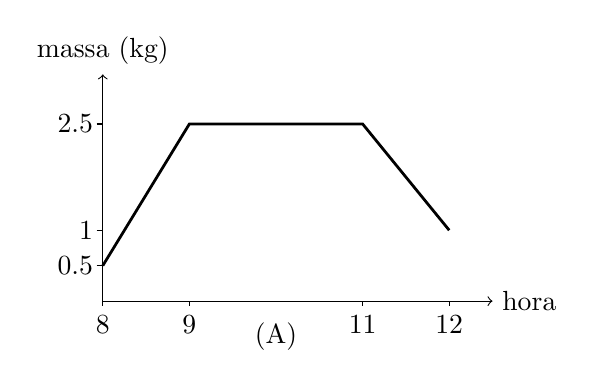
\begin{tikzpicture}[x=1.1cm,y=0.9cm]
    \draw[->] (0,0) -- (4.5,0) node[right] {hora};
    \draw[->] (0,0) -- (0,3.2) node[above] {massa (kg)};
    \draw[line width=1pt] (0,0.5) -- (1,2.5) -- (3,2.5) -- (4,1.0);
    \foreach \x/\lab in {0/8,1/9,3/11,4/12} \draw (\x,0) -- (\x,-0.07) node[below] {\lab};
    \foreach \y in {0.5,1,2.5} \draw (-0.07,\y) -- (0,\y) node[left] {\y};
    \node at (2,-0.5) {(A)};
\end{tikzpicture}
&
% Gráfico B (cresce continuamente)
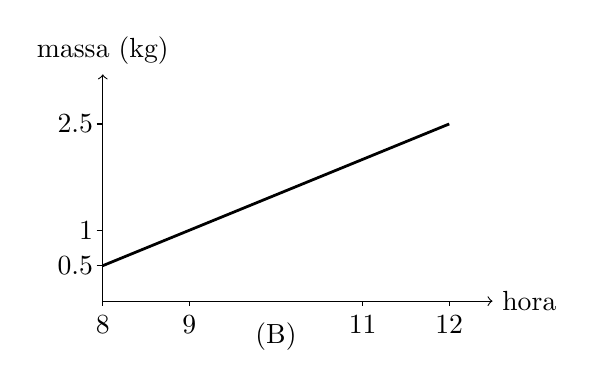
\begin{tikzpicture}[x=1.1cm,y=0.9cm]
    \draw[->] (0,0) -- (4.5,0) node[right] {hora};
    \draw[->] (0,0) -- (0,3.2) node[above] {massa (kg)};
    \draw[line width=1pt] (0,0.5) -- (4,2.5);
    \foreach \x/\lab in {0/8,1/9,3/11,4/12} \draw (\x,0) -- (\x,-0.07) node[below] {\lab};
    \foreach \y in {0.5,1,2.5} \draw (-0.07,\y) -- (0,\y) node[left] {\y};
    \node at (2,-0.5) {(B)};
\end{tikzpicture}
\\[8pt]
% Gráfico C (desce depois sobe)
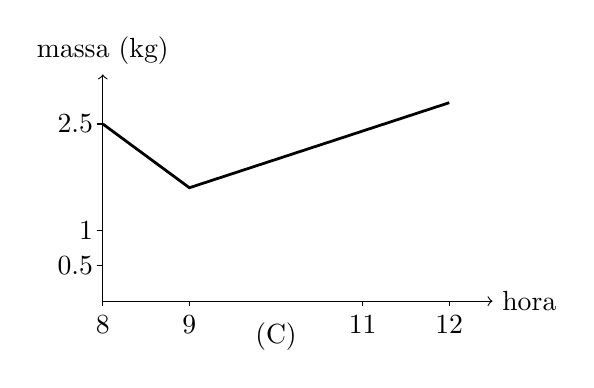
\begin{tikzpicture}[x=1.1cm,y=0.9cm]
    \draw[->] (0,0) -- (4.5,0) node[right] {hora};
    \draw[->] (0,0) -- (0,3.2) node[above] {massa (kg)};
    \draw[line width=1pt] (0,2.5) -- (1,1.6) -- (3,2.4) -- (4,2.8);
    \foreach \x/\lab in {0/8,1/9,3/11,4/12} \draw (\x,0) -- (\x,-0.07) node[below] {\lab};
    \foreach \y in {0.5,1,2.5} \draw (-0.07,\y) -- (0,\y) node[left] {\y};
    \node at (2,-0.5) {(C)};
\end{tikzpicture}
&
% Gráfico D (praticamente constante)
\begin{tikzpicture}[x=1.1cm,y=0.9cm]
    \draw[->] (0,0) -- (4.5,0) node[right] {hora};
    \draw[->] (0,0) -- (0,3.2) node[above] {massa (kg)};
    \draw[line width=1pt] (0,2.4) -- (4,2.4);
    \foreach \x/\lab in {0/8,1/9,3/11,4/12} \draw (\x,0) -- (\x,-0.07) node[below] {\lab};
    \foreach \y in {0.5,1,2.5} \draw (-0.07,\y) -- (0,\y) node[left] {\y};
    \node at (2,-0.5) {(D)};
\end{tikzpicture}
\end{tabular}
\end{center}
}

\subexercicio{Indique a letra do gráfico que considera correcta (A/B/C/D).}

\subexercicio{Justifique brevemente a sua escolha, referindo as partes do enunciado: "cresceu de ... a ...", "manteve-se aproximadamente constante" e "diminuiu de ... a ...".}
